\section{Διαμόρφωση Δικτύων Κωδικοποίησης Υψηλοσυχνοτικού Περιεχομένου}
\label{section:featureModulation}

Στα πλαίσια της διαμόρφωσης των δικτύων κωδικοποίησης, εντάσσονται όλες οι τεχνικές που ασχολούνται με την διαδικασία κανονικοποίησης των εξαγόμενων χαρακτηριστικών και έχουν να κάνουν συνήθως με το ποία χαρακτηριστικά ευνοεί και ποια τα χαρακτηριστικά το ρίχνει το δίκτυο. Μια ικανοποιητική ανακατασκευή απαιτεί κατά περίπτωση έκφραση όλων των χαρακτηριστικών που είναι απαραίτητα. Επομένως ακολουθούνται τεχνικές προσαρμοστικής κανονικοποίησης σε κάθε χαρακτηριστικό κατά την διάρκεια της εκπαίδευσης τα οποία περιγράφονται τόσο ως έμπνευση από εργασίες που ήδη χρησιμοποιούν αυτές τις τεχνικές με επιτυχία όπως το \enit{StyleGAN2} \cite{karras2020analyzing}. Στο κομμάτι της μεθοδολογίας που αναφέρεται πώς ακριβώς εφαρμόστηκε ο μηχανισμός αυτός που βασίστηκε περισσότερο στο έννοια της προσοχής. \cite{vaswani2023attention}.

\begin{figure}[H]
    \centering
    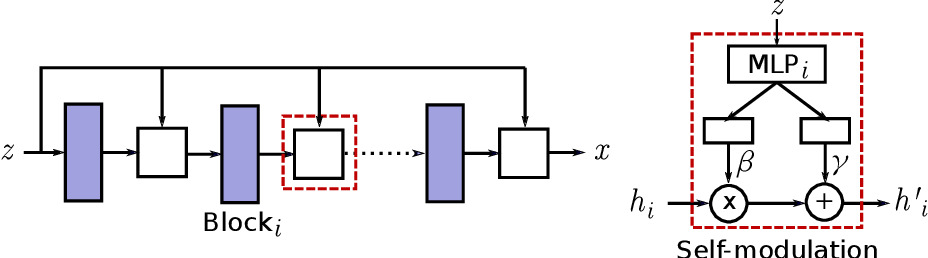
\includegraphics[width=0.4\linewidth]{images/chapter2_img/self-modulationMLPS.jpg}
    \caption{Αυτό-Διαμόρφωση MLP δικτύου, πηγή \cite{Chen2018OnSM}}
    \label{fig:selfmod}
\end{figure}